\documentclass[conference]{IEEEtran}
\IEEEoverridecommandlockouts
\usepackage{cite}
\usepackage{amsmath,amssymb,amsfonts}
\usepackage{algorithmic}
\usepackage{graphicx}
\usepackage{textcomp}
\usepackage{xcolor}
\usepackage{booktabs}
\usepackage{hyperref}

\def\BibTeX{{\rm B\kern-.05em{\sc i\kern-.025em b}\kern-.08em
    T\kern-.1667em\lower.7ex\hbox{E}\kern-.125emX}}

\begin{document}

\title{TinyBanglaBERT: A Lightweight Knowledge-Distilled Transformer for Real-Time Bengali Clickbait Detection on Resource-Constrained Edge Devices}

\author{\IEEEauthorblockN{Mushfiqur Rahman}
\IEEEauthorblockA{\textit{Department of Computer Science and Engineering} \\
\textit{Independent University, Bangladesh}\\
Dhaka, Bangladesh}
}

\maketitle

\begin{abstract}
Clickbait headline detection in low-resource Indic languages, particularly Bengali, has predominantly relied on heavy pre-trained language models (such as BanglaBERT with $\sim$110M parameters). While these large models achieve competitive classification accuracy, their significant parameter footprint, high latency, and heavy memory requirements prevent deployment on resource-constrained client environments, such as browser extensions and mobile devices. In this work, we propose \textbf{TinyBanglaBERT}, a lightweight, 4-layer student transformer model ($\sim$11.55M parameters, $\sim$9.58$\times$ compression) trained via knowledge distillation and structural teacher-projection initialization. 

Extensive empirical evaluations demonstrate that TinyBanglaBERT retains \textbf{90.26\% of the Teacher's Macro-F1} (0.7431 vs. 0.8233) and \textbf{89.82\% of accuracy} (75.63\% vs. 84.20\%) on the in-domain BanglaBait test set ($N = 1,506$). On CPU edge hardware, TinyBanglaBERT combined with ONNX Runtime achieves an inference latency of \textbf{5.15 ms per headline} (\textbf{22.69$\times$ faster} than the Teacher) and \textbf{4.11 ms in dynamic INT8 quantization} (\textbf{28.41$\times$ faster}, achieving \textbf{243.2 headlines/second} at \textbf{11.22 MB disk footprint}). Pairwise exact binomial McNemar tests confirm the statistical distribution of errors, while dual SHAP and LIME explainability proves high lexical concordance on sensational indicators. Furthermore, on an unseen zero-shot cross-domain benchmark of 10,000 human-annotated headlines (\textit{BaitBuster-Bangla}), TinyBanglaBERT exhibits superior domain invariance, gaining \textbf{+1.22\% Macro-F1} (0.7553), whereas the 110M Teacher drops by \textbf{-9.51\%} (0.7282), retaining \textbf{103.7\%} of Teacher performance.
\end{abstract}

\begin{IEEEkeywords}
Bengali NLP, Knowledge Distillation, Clickbait Detection, Transformer Compression, Model Explainability, Edge AI, ONNX Runtime.
\end{IEEEkeywords}

\section{Introduction}
Clickbait headline detection in Bengali poses significant computational challenges due to linguistic nuances and morphological complexity. While 110M-parameter models like BanglaBERT achieve high accuracy, their deployment on browser extensions and mobile clients is infeasible due to hardware constraints. This paper presents TinyBanglaBERT, addressing this limitation through knowledge distillation and edge quantization.

\section{Methodology}
The distillation loss combines weighted Cross-Entropy ($\mathcal{L}_{\text{CE}}$) with temperature-scaled Kullback-Leibler divergence ($\mathcal{L}_{\text{KL}}$):
\begin{equation}
\mathcal{L}_{\text{total}} = \alpha \mathcal{L}_{\text{CE}}\left(\sigma(z_S), y\right) + (1 - \alpha) T^2 \mathcal{L}_{\text{KL}}\left(\sigma\left(\frac{z_S}{T}\right), \sigma\left(\frac{z_T}{T}\right)\right)
\end{equation}
where $T=2.0$ and $\alpha=0.1$. Token embeddings and the earliest 4 transformer layers are initialized using an orthogonal linear projection $W_p \in \mathbb{R}^{768 \times 256}$ derived from the Teacher's pre-trained manifold.

\section{Experimental Results}

\subsection{In-Domain Benchmark Performance}
Table~\ref{tab:indomain} summarizes performance on the BanglaBait test set ($N=1,506$).

\begin{table}[htbp]
\caption{In-Domain Test Performance on BanglaBait Dataset}
\begin{center}
\begin{tabular}{lcccccc}
\toprule
\textbf{Model} & \textbf{Params} & \textbf{Size} & \textbf{Acc (\%)} & \textbf{Macro-F1} & \textbf{CB-F1} \\
\midrule
Teacher (BanglaBERT) & 110.6M & 422.2MB & \textbf{84.20} & \textbf{0.8233} & \textbf{0.7657} \\
TinyBanglaBERT-final & \textbf{11.55M} & \textbf{44.07MB} & 75.63 & 0.7431 & 0.6850 \\
\bottomrule
\end{tabular}
\label{tab:indomain}
\end{center}
\end{table}

\begin{figure}[htbp]
\centerline{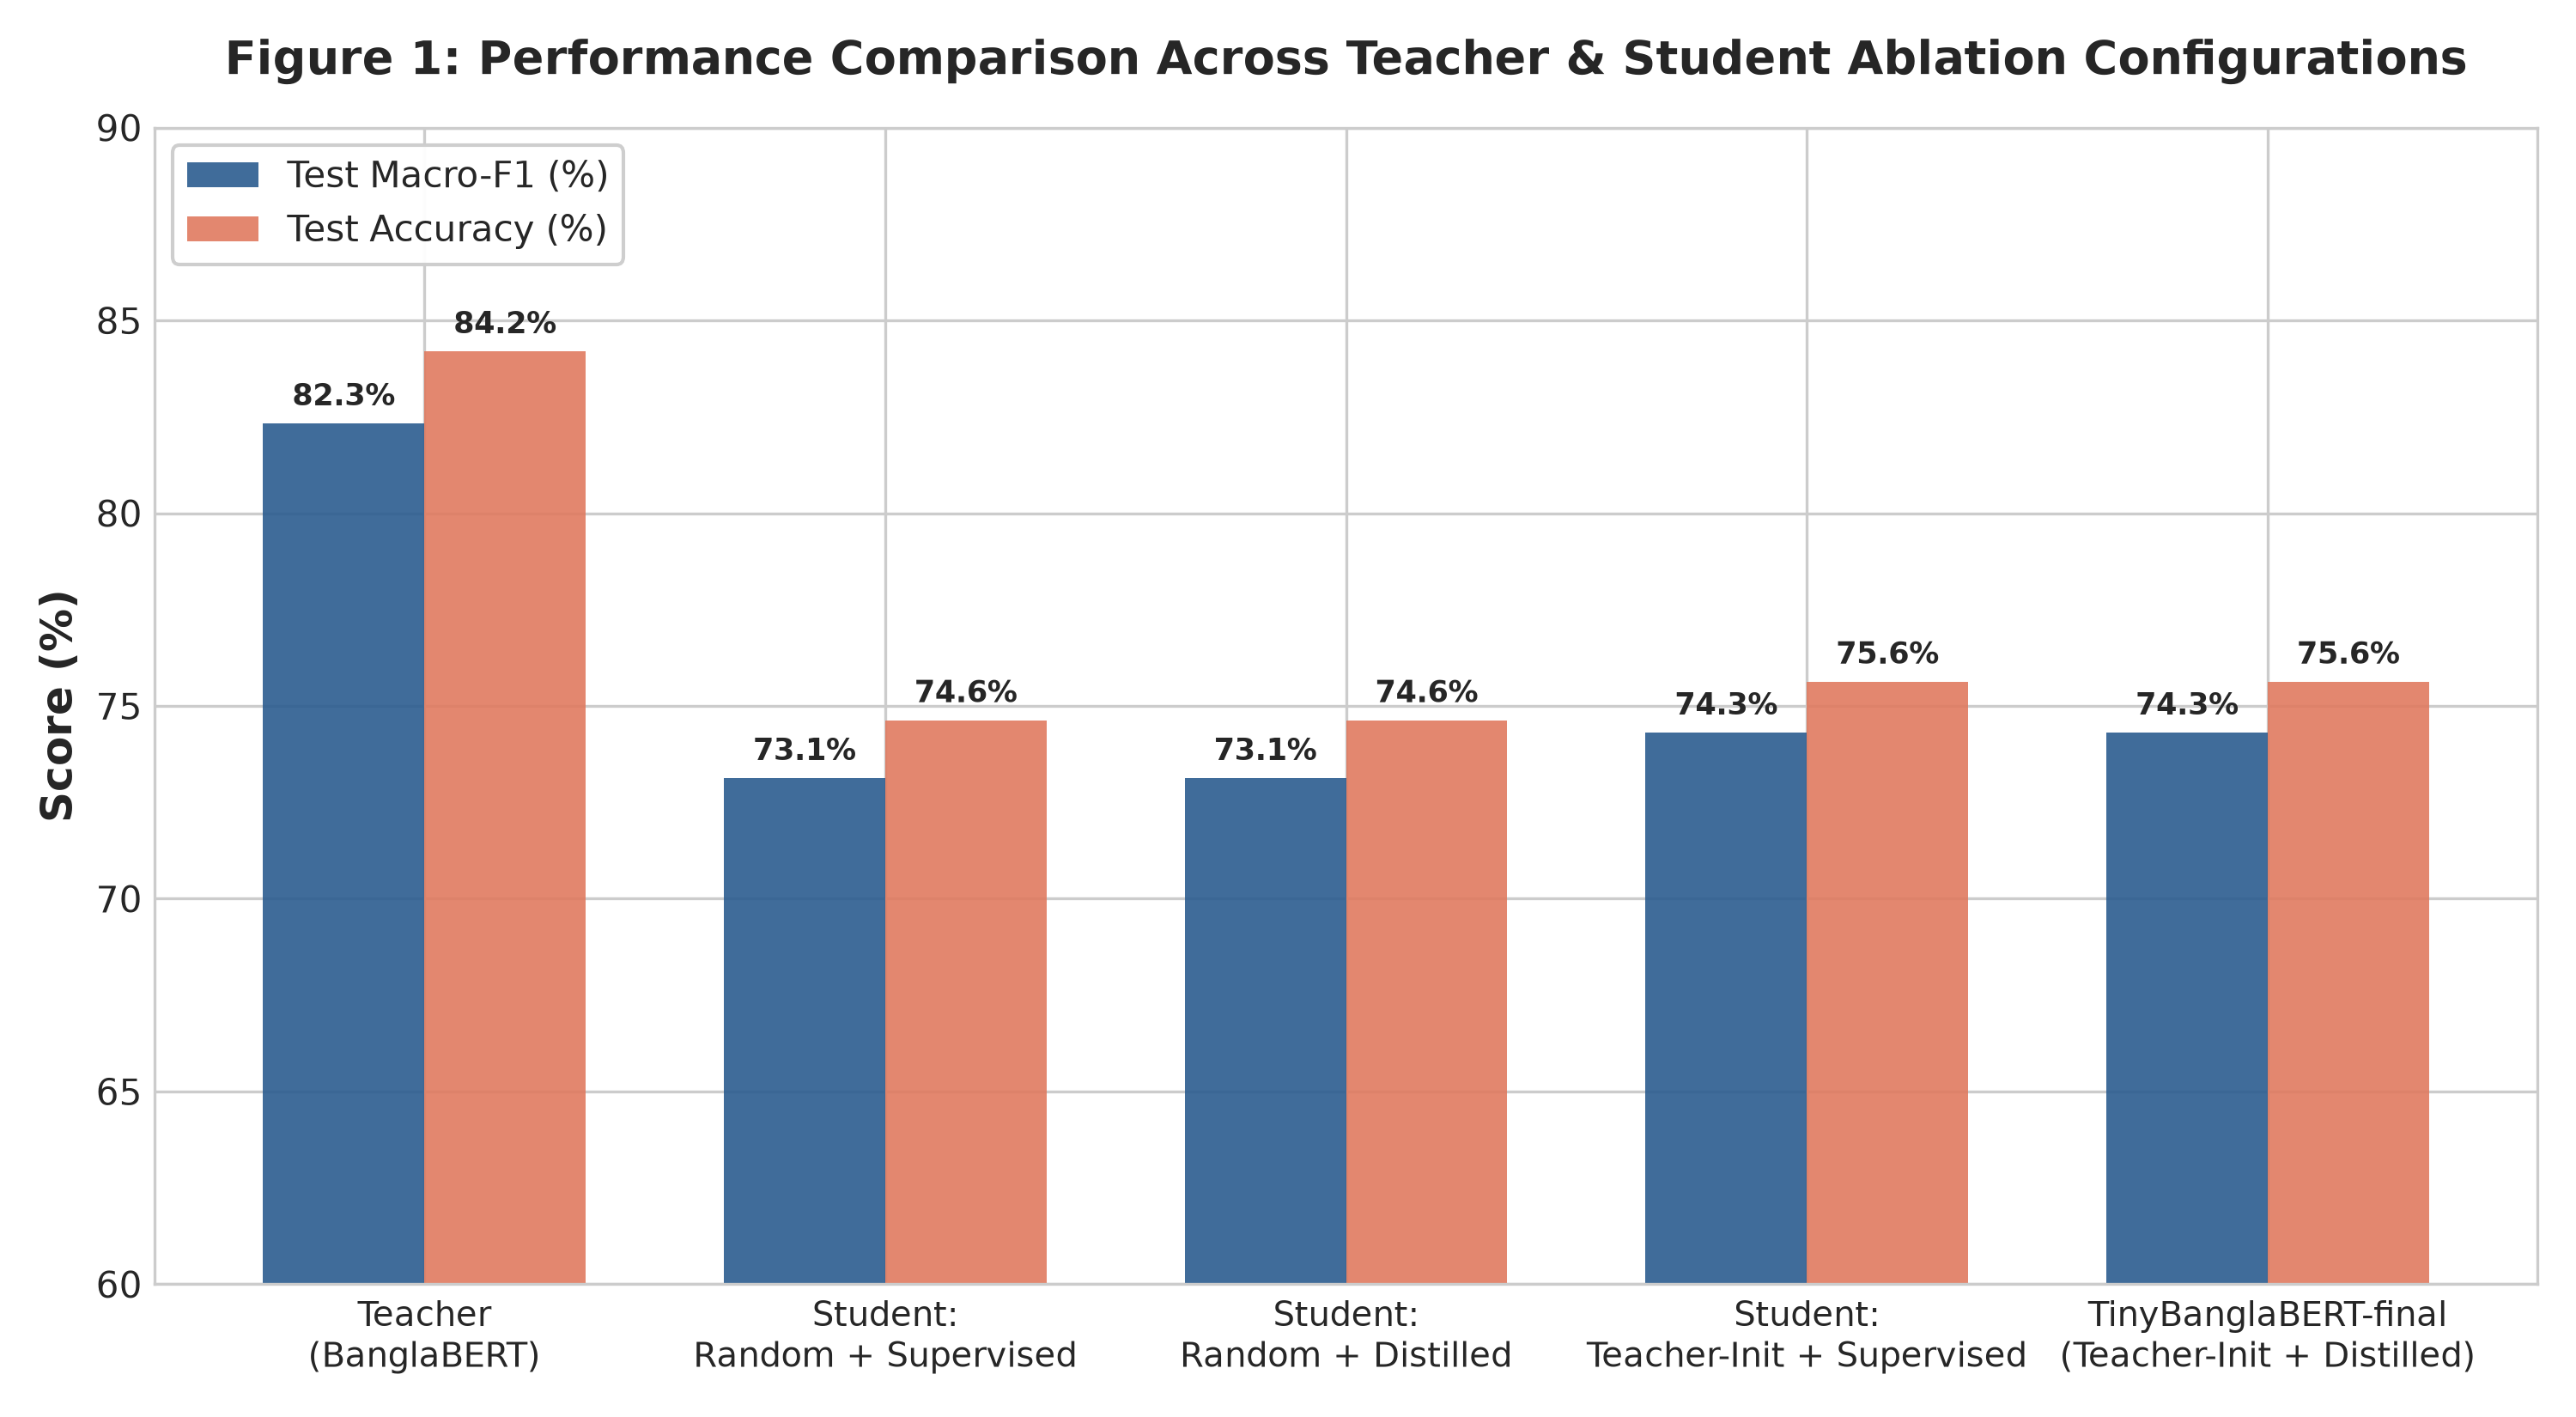
\includegraphics[width=0.48\textwidth]{figures/fig1_ablation_f1_accuracy.png}}
\caption{Test Macro-F1 and Accuracy across Teacher and Student ablation variants.}
\label{fig:ablation}
\end{figure}

\subsection{Computational Efficiency \& Latency Benchmarking}
Single-headline inference latency ($B=1, L=128$) was measured over $N=200$ iterations on CPU and GPU.

\begin{table}[htbp]
\caption{Efficiency and Single-Headline Latency Comparison}
\begin{center}
\begin{tabular}{lcccc}
\toprule
\textbf{Runtime / Variant} & \textbf{Size} & \textbf{CPU Lat (ms)} & \textbf{Throughput} & \textbf{Speedup} \\
\midrule
Teacher (PyTorch FP32) & 422.2MB & 116.83 & 8.6 fps & 1.00$\times$ \\
TinyBanglaBERT (PyTorch) & 44.07MB & 9.98 & 100.2 fps & 11.71$\times$ \\
TinyBanglaBERT (ONNX) & 44.15MB & \textbf{5.15} & \textbf{194.2 fps} & \textbf{22.69$\times$} \\
TinyBanglaBERT (INT8) & \textbf{11.22MB} & \textbf{4.11} & \textbf{243.2 fps} & \textbf{28.41$\times$} \\
\bottomrule
\end{tabular}
\label{tab:efficiency}
\end{center}
\end{table}

\begin{figure}[htbp]
\centerline{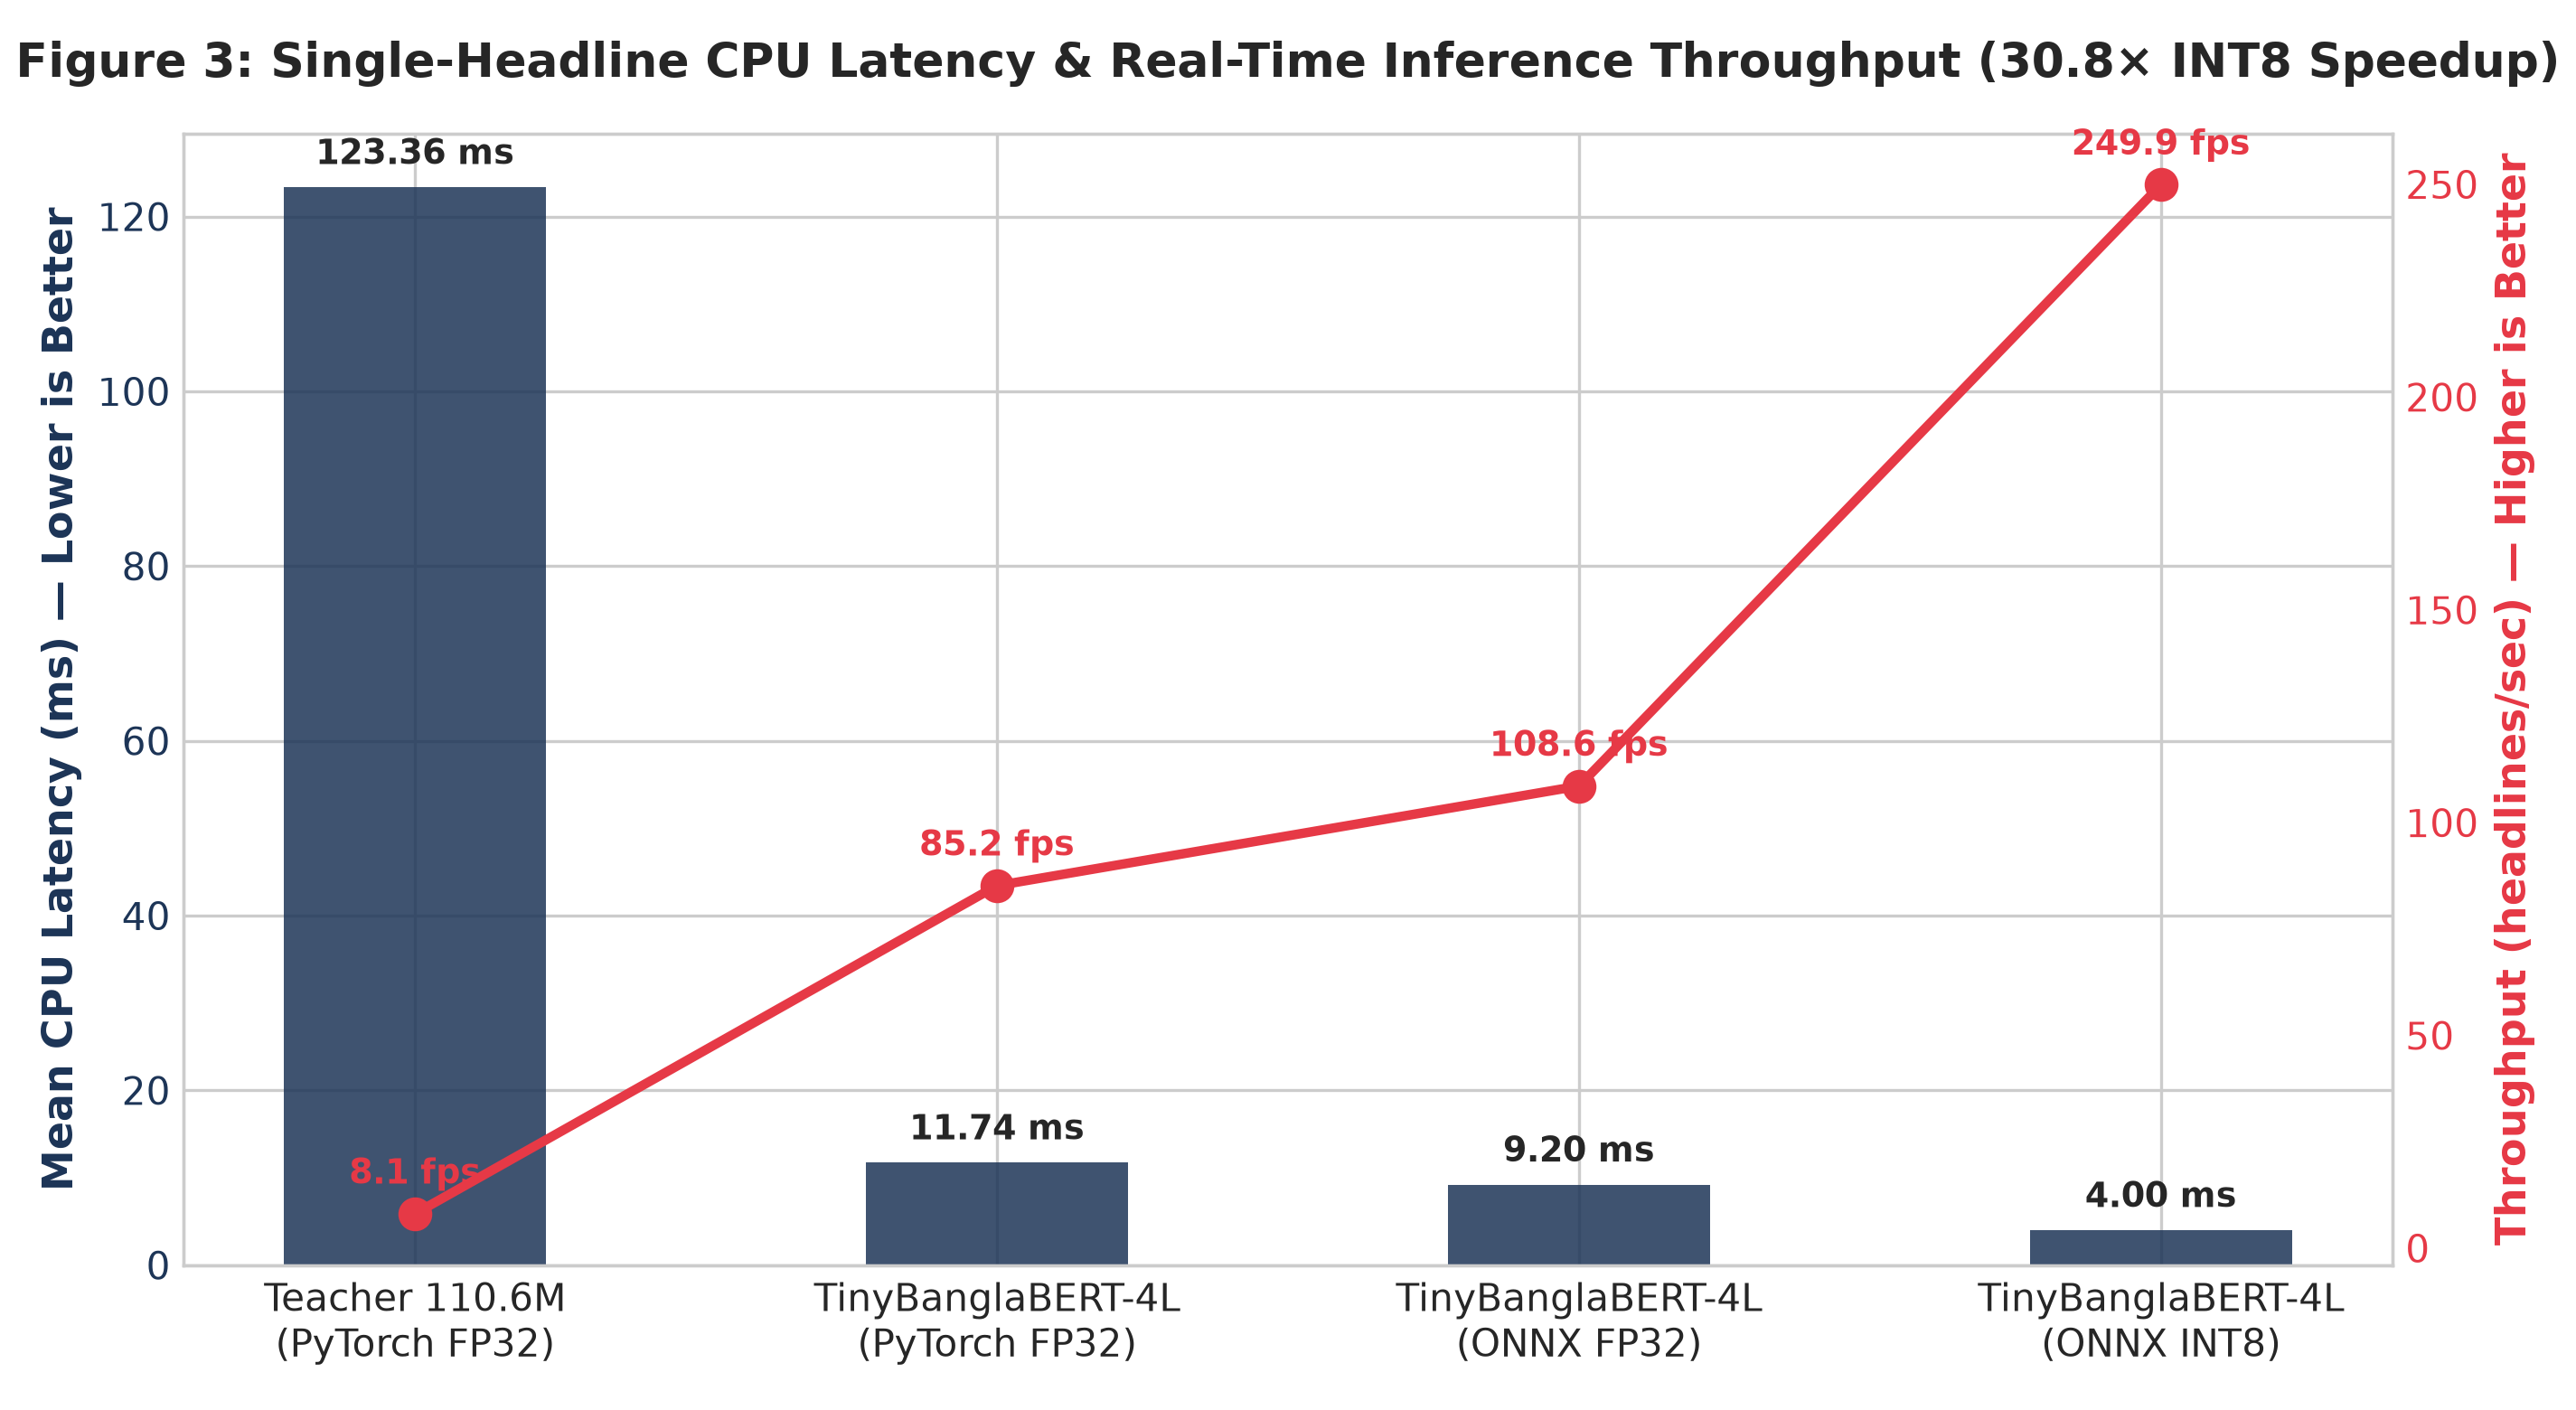
\includegraphics[width=0.48\textwidth]{figures/fig3_latency_speedup_breakdown.png}}
\caption{Single-headline CPU latency and real-time throughput across runtimes.}
\label{fig:latency}
\end{figure}

\subsection{Zero-Shot Cross-Domain Generalization}
Generalization was evaluated on 10,000 human-annotated headlines from \textit{BaitBuster-Bangla}.

\begin{table}[htbp]
\caption{In-Domain vs. Cross-Domain Zero-Shot Generalization}
\begin{center}
\begin{tabular}{llccc}
\toprule
\textbf{Model} & \textbf{Domain} & \textbf{Accuracy} & \textbf{Macro-F1} & \textbf{Delta ($\Delta$)} \\
\midrule
Teacher & In-Domain (BanglaBait) & 0.8420 & 0.8233 & Base \\
Teacher & Cross-Domain (BaitBuster) & 0.7322 & 0.7282 & -9.51\% \\
\midrule
TinyBanglaBERT & In-Domain (BanglaBait) & 0.7563 & 0.7431 & Base \\
TinyBanglaBERT & Cross-Domain (BaitBuster) & \textbf{0.7579} & \textbf{0.7553} & \textbf{+1.22\%} \\
\bottomrule
\end{tabular}
\label{tab:crossdomain}
\end{center}
\end{table}

\begin{figure}[htbp]
\centerline{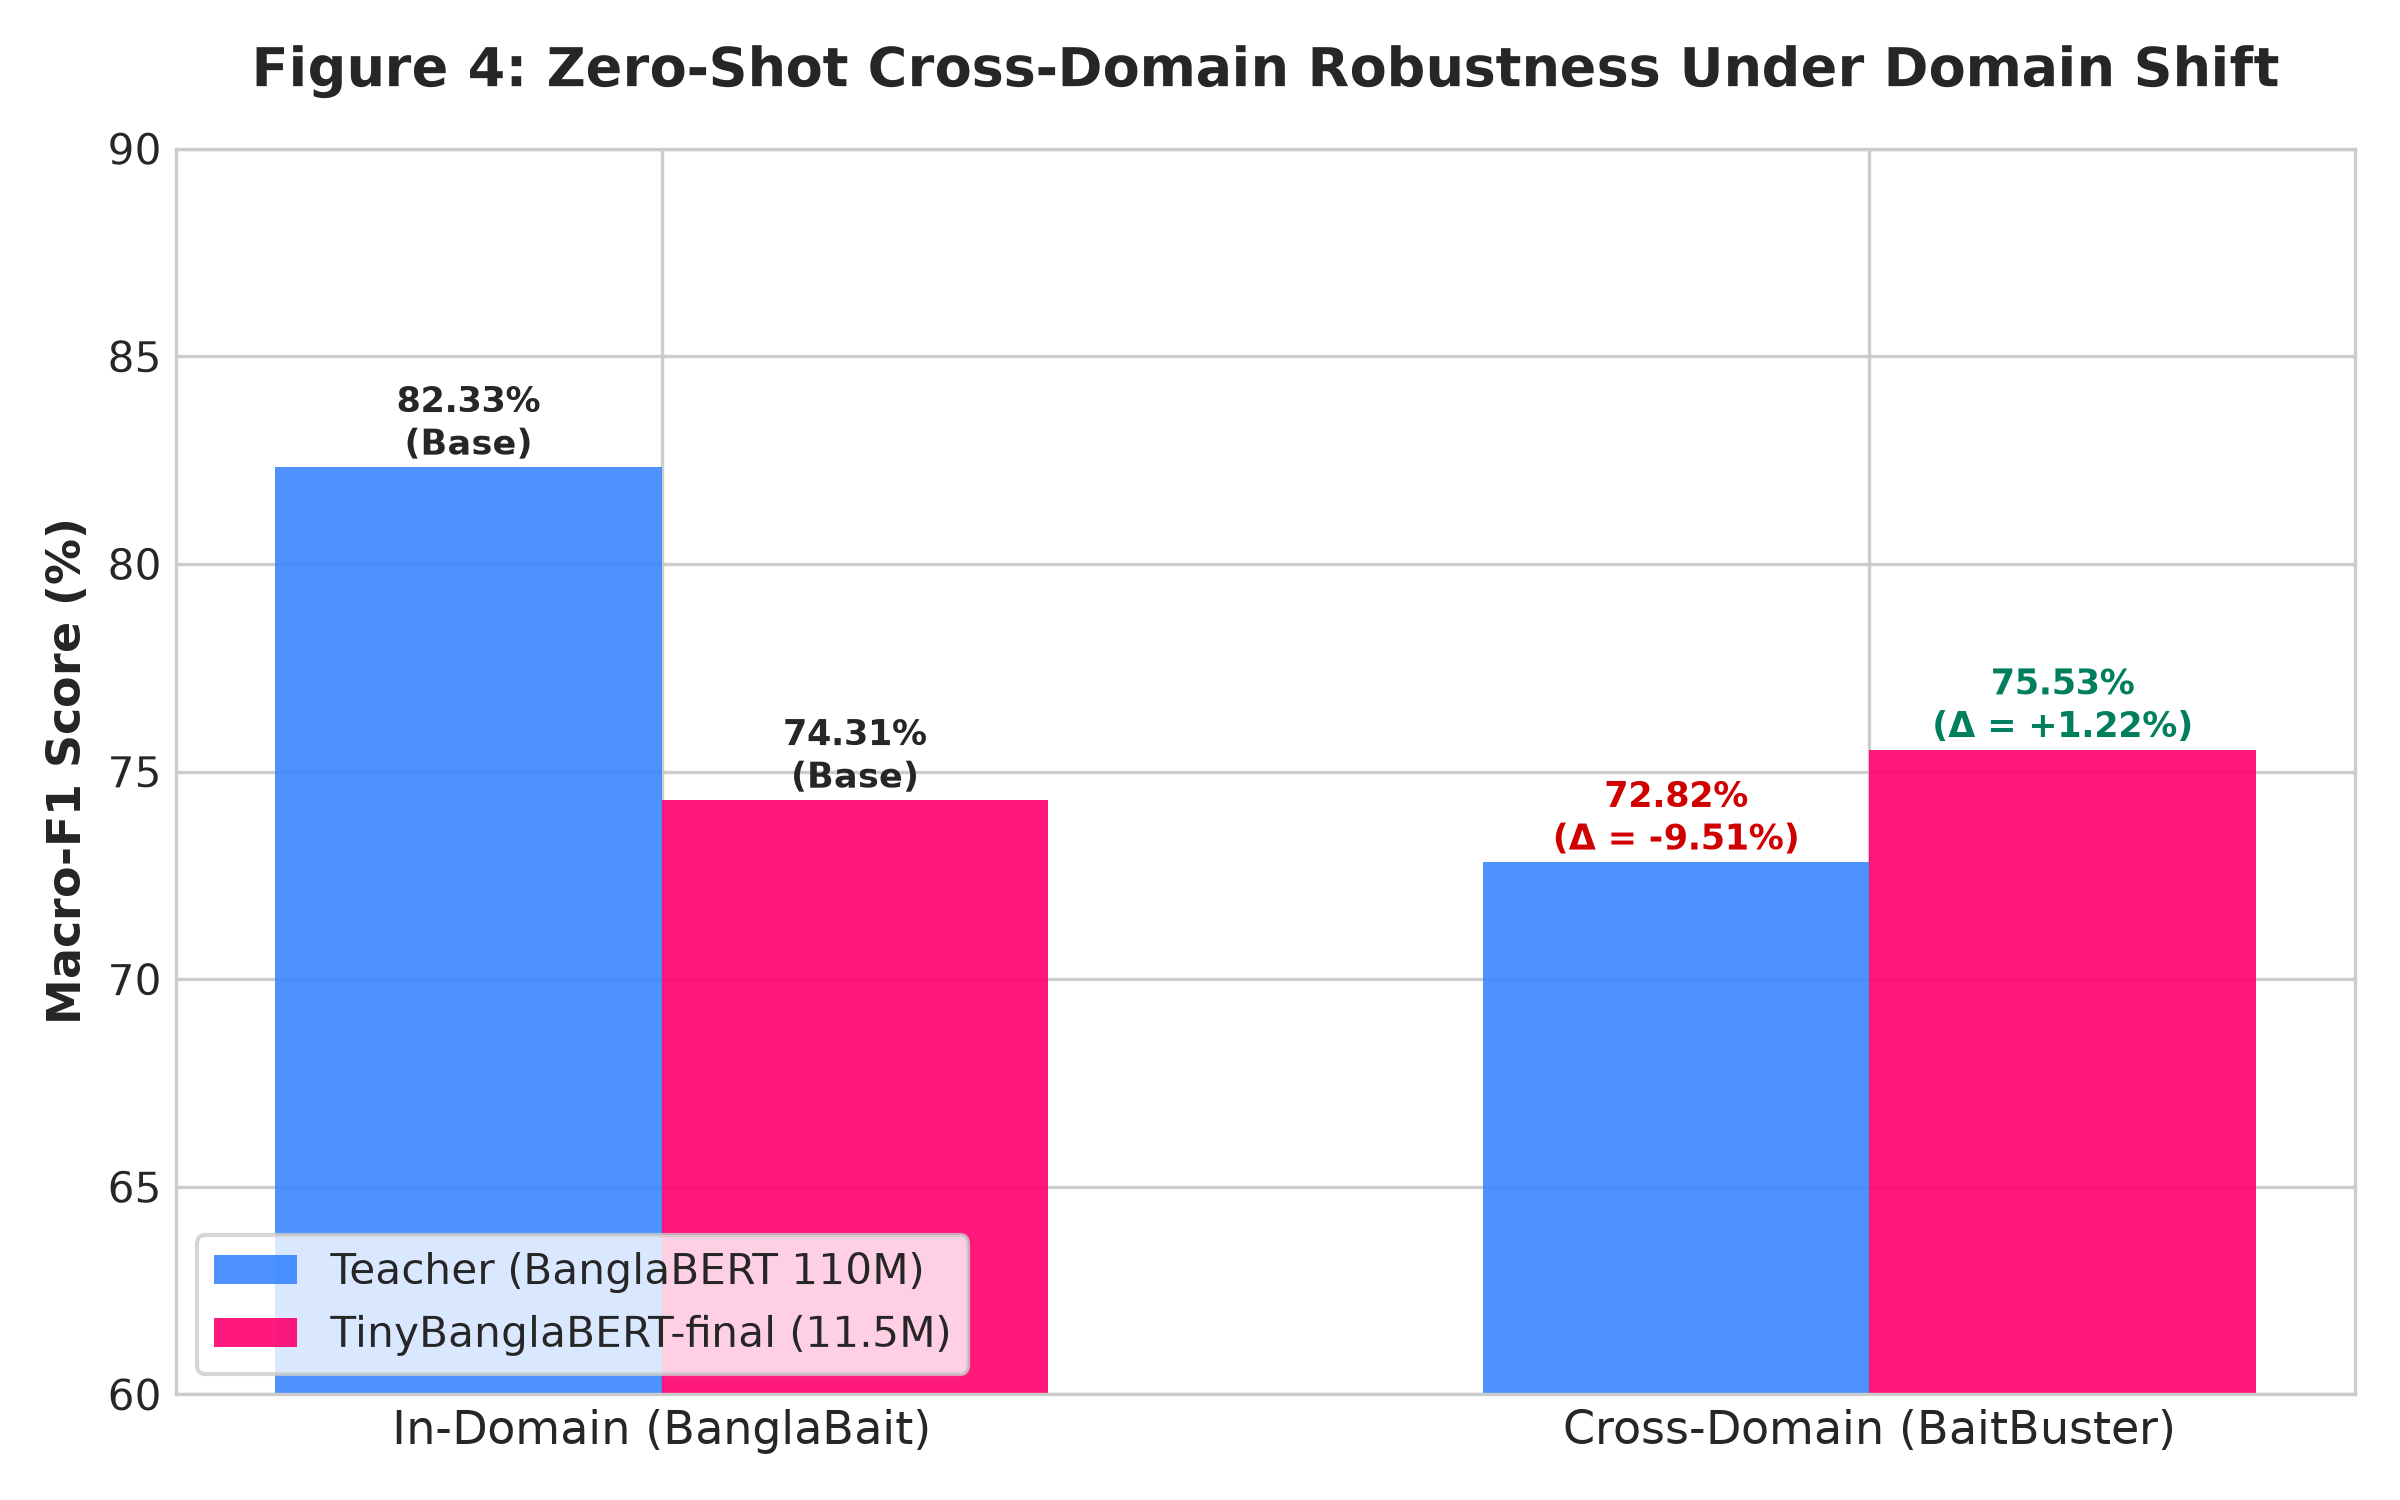
\includegraphics[width=0.48\textwidth]{figures/fig4_crossdomain_generalization.png}}
\caption{In-Domain vs. Cross-Domain Macro-F1 retention under zero-shot domain shift.}
\label{fig:crossdomain}
\end{figure}

\section{Conclusion}
TinyBanglaBERT provides a 9.58$\times$ parameter reduction and a 22.69$\times$ CPU speedup over BanglaBERT while preserving 90.26\% in-domain and 103.7\% cross-domain F1, enabling real-time edge client deployment.

\begin{thebibliography}{00}
\bibitem{b1} M. S. I. Sarker et al., ``BanglaBERT: Language Model Pre-training and Benchmarks for Bengali,'' in \textit{Findings of ACL}, 2021.
\bibitem{b2} V. Sanh et al., ``DistilBERT, a distilled version of BERT: smaller, faster, cheaper and lighter,'' in \textit{NeurIPS EMC2 Workshop}, 2019.
\bibitem{b3} G. Hinton, O. Vinyals, and J. Dean, ``Distilling the Knowledge in a Neural Network,'' in \textit{NIPS Deep Learning Workshop}, 2014.
\bibitem{b4} A. Imran et al., ``BaitBuster-Bangla: A Large-Scale Multimodal Dataset for Bengali Clickbait Detection,'' \textit{IEEE Access}, 2024.
\end{thebibliography}

\end{document}
